\section{Testes e Avaliação de Desempenho (\textit{Benchmarking})}
\label{subsec:validacao-ascon}
\subsection{\textit{Known Answer Tests} (KAT)}
A primeira etapa é a validação através dos \textit{Known Answer Tests} (KAT), que são testes disponibilizados pelo próprio grupo que desenvolveu o Ascon. Eles fornecem parâmetros de entrada específicos que devem resultar em saídas exatas e já esperadas. Como o trabalho utiliza a variante Ascon-128a (versão 1.2), a validação emprega os vetores de teste correspondentes a essa versão, distribuídos junto à própria \textit{ascon-suite} e derivados do repositório de referência \textit{ascon-c} \cite{ascon_reference_c}.

Para validar a biblioteca de forma puramente matemática, os testes são rodados exaustivamente em um computador desktop. Depois, para garantir que não haja nenhuma anomalia de compilação ou diferença causada pela arquitetura de hardware, testes adicionais são executados diretamente na placa, com um volume menor de vetores.

Como garantia extra, a validação na placa precede qualquer coleta de desempenho, de modo que as medições incidam apenas sobre uma implementação já verificada, o próprio \textit{firmware} de medição repete dois vetores do KAT, e um vetor de referência do AES-GCM, antes de medir, e interrompe a execução se algum deles falhar. Ao comparar as saídas das funções da biblioteca \textit{ascon-suite} com os resultados oficiais, comprova-se de forma prática que a implementação opera corretamente no ambiente do projeto.

%%%%%%%%%%%%%%%%%%%%%%%%%%%%%%%%%%%%%%%%%%%%%%%%%%%%

\subsection{Validação dos Dados Associados (AEAD)}
Outro teste é a validação da autenticidade do modo AEAD e a sua capacidade de rejeição de anomalias. Para avaliar a resiliência do sistema contra um ataque de \textit{Man-in-the-middle} (MitM), no qual um interceptador tenta forjar ou corromper a mensagem em trânsito, a metodologia emprega a técnica de injeção intencional de falhas (\textit{bit-flipping}).

Após a geração de um pacote válido, o firmware de teste altera intencionalmente bits específicos antes de repassar a mensagem para a função de decifragem. A adulteração é testada em três frentes distintas.
\begin{itemize}
\item \textbf{No texto cifrado (\textit{Ciphertext}):} simulando um atacante que tenta alterar o valor do \textit{payload} do sensor.
\item \textbf{Nos Dados Associados (AD):} alterando o cabeçalho do protocolo LoRaWAN, simulando uma tentativa de modificar metadados de roteamento ou de identificação do nó.
\item \textbf{Na \textit{Tag} de Autenticação:} simulando um cenário onde a mensagem é modificada e o atacante anexa uma assinatura forjada ou corrompida.
\end{itemize}

O resultado esperado em todos os cenários de adulteração é que a função de decifragem do algoritmo reconheça a quebra de integridade e falhe imediatamente, retornando um código de erro e garantindo que nenhum fragmento do texto claro modificado seja entregue para a camada de aplicação do microcontrolador.

%%%%%%%%%%%%%%%%%%%%%%%%%%%%%%%%%%%%%%%%%%%%%%%%%%%%

\subsection{Vazamento de Memória e Ataques de Canal Colateral}
A avaliação de desempenho não se limita à validação funcional e engloba também o consumo de memória (RAM) e o tempo de execução. Para a análise de memória, a metodologia emprega as funções nativas do ESP-IDF. O uso do \textit{Heap} é monitorado por meio da função \texttt{esp\_get\_free\_heap\_size()} antes e depois da execução e, durante a execução, por uma tarefa no segundo núcleo do processador que lê o \textit{heap} livre continuamente e registra o menor valor observado, de modo a detectar alocações feitas e liberadas dentro da própria operação, invisíveis à comparação entre o antes e o depois. Adicionalmente, mede-se a profundidade máxima alcançada na Pilha (\textit{Stack}) através da função \texttt{uxTaskGetStackHighWaterMark()}, lida dentro de uma tarefa dedicada à operação, uma vez que essa marca registra o ponto mais fundo já atingido pela pilha da tarefa, lida na tarefa principal ela refletiria o uso anterior de outras rotinas, e não o do algoritmo.

Outro aspecto avaliado é o espaço ocupado de memória. O procedimento consiste em compilar o firmware e analisar o uso de memória Flash, comparando os resultados do compilador com e sem a inclusão da biblioteca no projeto.

Quanto ao tempo de execução, a metodologia busca não apenas medir a eficiência, mas também validar a resistência das implementações contra ataques de canal colateral baseados em tempo (\textit{Timing Side-Channel Attacks}). A medição extrai diretamente a quantidade de ciclos de \textit{clock} processados, lendo o contador de ciclos da CPU do ESP32 por meio da função \texttt{ESP.getCycleCount()}, para a cifragem e para a decifragem, em \textit{payloads} de 0, 2, 16, 23, 32 e 64 bytes. Os múltiplos de 16 bytes sustentam o modelo linear de custo por bloco, o \textit{payload} vazio mede a parcela fixa diretamente, e 2 e 23 bytes correspondem aos dois tamanhos de mensagem que ocorrem no \textit{dataset} Tour Perret, usado pela frente de aprendizado de máquina. Em cada tamanho é tomado o piso, o menor valor de 2.000 medidas, com as interrupções habilitadas, de modo que Ascon e AES sejam medidos exatamente da mesma forma. O \textit{driver} de AES do ESP-IDF já protege a operação de bloco com uma seção crítica própria \cite{espressif2026idf}, e o piso de 2.000 medidas faz o papel de filtro contra as interrupções que atingem o restante da chamada. Para o Ascon, o piso com as interrupções desabilitadas é medido como contraprova. Para validar a mitigação de ataques de canal colateral, são realizados testes repetitivos enviando cargas de dados (\textit{payloads}) com conteúdos e chaves completamente distintos, mas de tamanhos idênticos, incluindo classes de entrada fixas (todos os bytes nulos, todos 0xFF, alternados) e variáveis (rampa e valores derivados de um \textit{hash}), na linha do método dudect, que compara o tempo entre classes de entrada em vez de confiar numa única distribuição \cite{reparaz2017dudect}. O resultado esperado é que a variação nos ciclos de \textit{clock} consumidos seja desprezível, coerente com o projeto do algoritmo. A camada de substituição do Ascon dispensa tabelas de consulta, o que afasta ataques de temporização por cache \cite{ascon_v12_spec}. Dessa forma, o tempo de processamento do nó sensor não permite ao atacante deduzir fragmentos da chave ou da mensagem.

Por fim, para verificar a reprodutibilidade, o procedimento é repetido em 100 execuções independentes por tamanho de \textit{payload}, registrando-se o piso de ciclos (o menor valor medido) de cada execução, nas duas placas do projeto, o ESP32 clássico e o ESP32-S3 da placa Heltec com LoRa. A análise distingue a variação entre execuções, dada pela dispersão dos pisos, da variação interna a cada execução, dada pelo desvio padrão de suas medidas. O mesmo se aplica ao comparativo com o AES-128-GCM, tomando como métrica a razão entre os pisos, que cancela fatores comuns às duas medições.

%%%%%%%%%%%%%%%%%%%%%%%%%%%%%%%%%%%%%%%%%%%%%%%%%%%%

\subsection{Avaliação de Consumo Energético}
\label{subsec:energia_metodo}
A avaliação restringe-se ao custo energético das operações criptográficas, não incluindo o consumo da transmissão via rádio. A medição é realizada através da técnica de monitoramento da queda de tensão em um resistor de precisão (\textit{shunt}) de 1$\Omega$ conectado em série com a alimentação de 3,3V do microcontrolador \cite{hubble2024esp32power}, conforme a Figura~\ref{fig_setup_consumo}. As capturas são feitas com um osciloscópio digital, utilizando um pino GPIO como sinal de gatilho (\textit{trigger}) para delimitar com precisão o intervalo de tempo exato da execução das funções criptográficas.

Considerando que o módulo \textit{ESP32 DevKitV1} possui componentes periféricos que consomem corrente de forma constante, como o LED de operação, o regulador de tensão LDO e o conversor USB-Serial, a análise não foca no consumo absoluto da placa. Em vez disso, é aplicada a metodologia de Diferença de Consumo ($\Delta$), na qual subtrai-se a corrente de repouso (\textit{baseline}) do sistema ocioso do valor obtido durante o processamento do algoritmo.

Uma operação isolada não é mensurável dessa forma. A cifragem de 23 bytes dura cerca de 27~$\mu$s, e um acréscimo de poucos miliampères nesse intervalo desaparece no ruído da corrente de repouso da placa, da ordem de 50~mA, com a resolução de 8 bits do osciloscópio. Por isso cada operação é repetida 20.000 vezes em sequência, com o pino de gatilho em nível alto durante toda a rajada, que dura de meio segundo a dois segundos conforme o algoritmo e a placa. O osciloscópio registra a rajada inteira, e toma-se a média da tensão no resistor dentro da janela da rajada e a média em um trecho de repouso da mesma captura. A diferença entre as duas, dividida pela resistência, é a corrente que a operação acrescenta, e a energia por operação é o produto da tensão na placa, desse acréscimo e da duração da rajada, dividido pelo número de repetições. Além do Ascon-128a e do AES-128-GCM, em cifragem e decifragem, mede-se um caso de controle em que o processador apenas aguarda o mesmo tempo em um laço, para separar o custo de manter o núcleo ativo do custo do algoritmo. Durante a medição a placa é alimentada apenas pela fonte, com o cabo USB desconectado, porque o regulador da placa e o terra do cabo criariam caminhos de corrente por fora do resistor.

\begin{figure}[htb]
  \caption{\label{fig_setup_consumo}Configuração de medição de corrente via resistor \textit{shunt} e osciloscópio}
  \begin{center}
      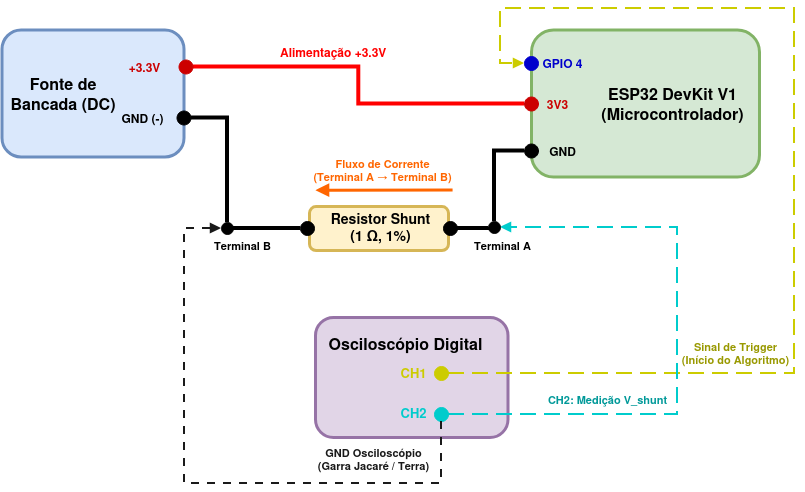
\includegraphics[scale=0.5]{felipe/figuras/setup_consumo_energia.png}
  \end{center}
  \legend{Fonte: Elaborado pelos autores (2026) com base em \cite{hubble2024esp32power}}
\end{figure}
